%!TEX root = ../main.tex
\chapter{Contribution}\label{chap:contribution}
\section{Notation}
In the following we will use the notation:
\begin{align*}
	\mathbb{I} \left(X , Y; D, P_M, C_M \right)
\end{align*}
which expresses the mutual information between $X$ and $Y$ and $D, P_M, C_M$, separated by a semi-colon, are the trainable parameters of the system. $D$ stands for the posterior probability distribution learnt by the demapper, $P_M$ stands for the source's probability distribution learnt by the encoder, and $C_M$ stands for the spatial distribution of the constellation points learnt by the mapper. These parameters can be seen as additional input to a function.

\section{First implementation}
In this section we break-down the autoencoder system presented by \citet{Stark}.
\subsection{Optimization of trainable parameters}
As we have seen in Chapter \ref{chap:preliminaries}, the goal of probabilistic constellation shaping is to maximize the \cgls{mi}. To this end, defining an appropriate loss function is critical. Starting from the demodulator, the categorial cross entropy loss
\begin{align}
	L(D, P_M, C_M) \triangleq \mathbb{X}(P_{X|Y}||Q_{X|Y}; D) = \mathbb{E}\left[-\log_2(Q(X|Y;D))\right] 
\end{align}

is appropriate for training $D$, but not for $P_M$ and $C_M$. A modification of this loss function is necessary to ensure that the end-to-end \cgls{mi} is maximized. The following expansions will come handy
\begin{align}
	\mathbb{H}(X) = \mathbb{X}(P_{X|Y}||Q_{X|Y}) - \mathbb{D}(P_{X|Y}||Q_{X|Y})
\end{align}
\begin{align}
	\mathbb{H}(X|Y=y) = \mathbb{X}(P_{X|y}||Q_{X|y}|Y=y) - \mathbb{D}(P_{X|y}||Q_{X|y}|Y=y)
\end{align}
\begin{align}
	\mathbb{H}(X|Y) = \mathbb{E}_y\left[\mathbb{X}(P_{X|y}||Q_{X|y}|Y=y)\right] - \mathbb{E}_y \left[\mathbb{D}(P_{X|y}||Q_{X|y}|Y=y)\right].
\end{align}
Using the last expansion we can rewrite the mutual information in terms of the categorical cross entropy
\begin{align}
	\mathbb{I} \left(X , Y\right) = \mathbb{H}(X) - \mathbb{X}(P_{X|Y}||Q_{X|Y}) + \mathbb{D}(P_{X|Y}||Q_{X|Y}).
\end{align}
And the categorical cross entropy loss function becomes 
\begin{align}
	L(D, P_M, C_M) \triangleq \mathbb{H}(X) - \mathbb{I} \left(X , Y\right) + \mathbb{D}(P_{X|Y}||Q_{X|Y}).
\end{align}
So, if $L$ is minimized during training, the source entropy is unwantedly minimized. To avoid this effect, \citeauthor{Stark} modify the loss function as
\begin{align}
	\hat{L}(D, P_M, C_M) \triangleq L(D, P_M, C_M) - \mathbb{H}(X).
\end{align}
With this correction the optimization problem 
\begin{align}
	\min_{D, P_M, C_M}\hat{L}(D, P_M, C_M) = \max_{D, P_M, C_M} \{ \mathbb{I} \left(X , Y\right) - \mathbb{D}(P_{X|Y}||Q_{X|Y})\}
\end{align}
maximizes the \cgls{mi}.
\subsection{Autoencoder Architecture}
\citeauthor{Stark}'s autoencoder is made up from three major blocks: sampler, modulator, and demodulator. Fig \ref{fig:starkAe} shows the complete architecture of the end-to-end system. While the modulator and demodulator blocks are similar to the proposal from \cite{O'Shea}, the simultaneous probabilistic shaping is possible thanks to the careful design of the sampler. By ensuring that the sampler mechanism is differentiable, the gradients with respect to each $p_i \in P_M$ are precise when calculated via \cgls{sgd}. In fact, the differentiability is gained by leveraging the so-called \textit{Gumbel-Softmax trick} \cite{JANG}, which circunvents the need for using the arg-max function to sample the discrete distribution $P_M$.

\begin{figure}[h]
	\includegraphics[width=\textwidth]{figs/stark_diagram.pdf}
	\centering	
	\caption{Proposed Autoencoder Architecture from \cite{Stark}}
	\label{fig:starkAe}
\end{figure}

\subsection{Autoencoder Performance}
We have implemented the end-to-end system using \cite{PyTorch}. First, for the 

\begin{figure}[h]
    \centering
    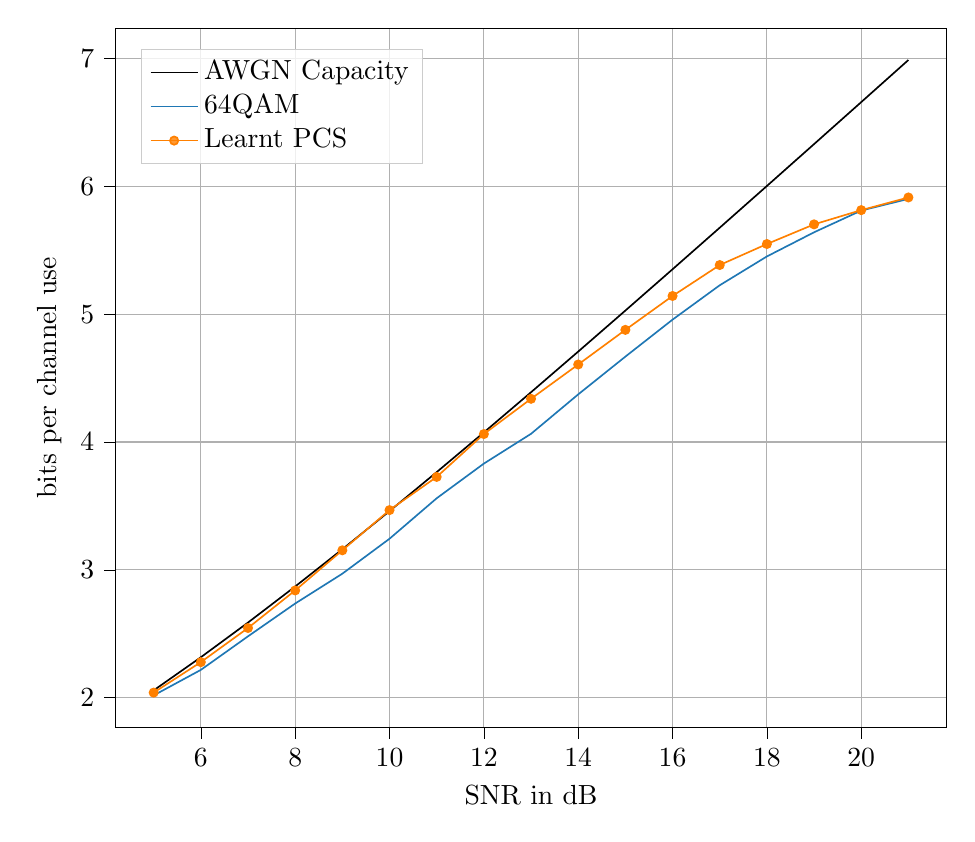
\begin{tikzpicture}

	\definecolor{darkgray176}{RGB}{176,176,176}
	\definecolor{lightgray204}{RGB}{204,204,204}
	\definecolor{steelblue31119180}{RGB}{31,119,180}
	
	\begin{axis}[
	width=\textwidth,
	legend cell align={left},
	legend style={
	  fill opacity=0.8,
	  draw opacity=1,
	  text opacity=1,
	  at={(0.03,0.97)},
	  anchor=north west,
	  draw=lightgray204
	},
	tick align=outside,
	tick pos=left,
	x grid style={darkgray176},
	xlabel={SNR in dB},
	xmajorgrids,
	xmin=4.2, xmax=21.8,
	xtick style={color=black},
	y grid style={darkgray176},
	ylabel={bits per channel use},
	ymajorgrids,
	ymin=1.76962706763051, ymax=7.23593185854285,
	ytick style={color=black}
	]
	\addplot [semithick, black]
	table {%
	5 2.0573732086068
	6 2.31645617962626
	7 2.58781437356203
	8 2.86978721917029
	9 3.16080442391302
	10 3.4594316186373
	11 3.76439436704286
	12 4.07458523490543
	13 4.38905896736305
	14 4.70702026272884
	15 5.02780767335052
	16 5.3508761542486
	17 5.67577990180488
	18 6.00215644400198
	19 6.32971245944191
	20 6.65821148275179
	21 6.98746345895592
	};
	\addlegendentry{AWGN Capacity}
	\addplot [semithick, steelblue31119180]
	table {%
	5 2.01809546721744
	6 2.2175518041323
	7 2.48006287743269
	8 2.73666019981578
	9 2.96994524819285
	10 3.24327265396585
	11 3.5599180244894
	12 3.83101129721386
	13 4.06389271002028
	14 4.37223116602331
	15 4.66762749613217
	16 4.95687064214095
	17 5.22562719816465
	18 5.4510408658335
	19 5.63991104919193
	20 5.80998181551279
	21 5.90102244617771
	};
	\addlegendentry{64QAM}
	\addplot [semithick, orange, mark=*, mark size=1.5, mark options={solid}]
	table {%
	5 2.0399120192814
	6 2.27815477000743
	7 2.545269624195
	8 2.83913156421006
	9 3.15282104007778
	10 3.46721977239767
	11 3.72686335626646
	12 4.06197533509096
	13 4.33772578214366
	14 4.60597916147994
	15 4.87677306853477
	16 5.14192078516177
	17 5.38382229480225
	18 5.54814724615274
	19 5.70199948596159
	20 5.81331697655905
	21 5.9123535300237
	};
	\addlegendentry{Learnt PCS}
	\end{axis}
	
	\end{tikzpicture}
	\caption{Mutual information learned by the probabilistic constellation shpaing on the AWGN channel.}
	\label{fig:starkPerf}
\end{figure}
	


\section{Second implementation}
In this section we break-down the autoencoder system presented by Aref et. al. in \cite{Aref}. This approach is motivated by the fact that the implementation presented by Stark et.al. presents numerical instabilities.

\subsection{Optimization of trainable parameters}
As we have seen in chapter \ref{chap:preliminaries}, the goal of probabilistic constellation shaping is to maximize the mutual information
\begin{align}
	 \max_{D, P_M, C_M} \mathbb{I} \left(X , Y ; D, P_M, C_M \right) = \mathbb{H}(X) - \mathbb{X}(P_{X|Y} \Vert Q_{X|Y} ; D, P_M, C_M)
\end{align}

where the entropy is maximized when the symbols probabilities follow a \cgls{mb} distribution; and the cross-equivocation is minimum when $Q_{X|Y} = P_{X|Y}$.

Typically, the gradient descent (or ascent, as we intent to maximize) allows us to solve the optimization problem by adjusting the trainable parameters as:
\begin{align}
	\theta_{new} = \theta_{old} + \epsilon \pdv{\theta_{old}} \mathbb{I} \left(X , Y ; \theta_{old} \right)
\end{align}
for all trainable parameters $\theta \in P_M, C_M, D$. And the \cgls{mi} can be numerically approximated by
\begin{align}
	\mathbb{I} \left(X , Y\right) \approx \mathbb{I} \left(X , Y\right)_{\text{num}} &= \dfrac{1}{B} \sum \limits_{i = 1}^{B} - \log_2(P(x_i)) + \log_2(Q_{X|Y}(x_i|y_i))\\
	&= \dfrac{1}{B} \sum \limits_{i = 1}^{B} L(x_i, y_i).
\end{align}

Next, the following approximation usually allows to adjust the trainable parameters:
\begin{align}
	\pdv{\theta} \mathbb{I} \left(X , Y ; \theta \right) \approx \pdv{\theta} \mathbb{I} \left(X , Y\right)_{\text{num}} = \dfrac{1}{B} \sum \limits_{i = 1}^{B} L(x_i, y_i).
\end{align}

However, Aref claims that although this is true for the constellation locations $(\theta \in C_M)$ and the demapper parameters $(\theta \in D)$, it does not hold for the constellation probabilities $\{p_1, p_2, \dots, p_M\} = P_M$
\begin{align}
\label{eqn:mi_pdv_p}
	\pdv{p_j} \mathbb{I} \left(X , Y ; P_M \right) \not\approx \dfrac{1}{B} \sum \limits_{i = 1}^{B} \pdv{p_j} L(x_i, y_i)
\end{align}

as $\{p_1, p_2, \dots, p_M\}$ changes the statistics of the training set.

For this reason, (\ref{eqn:mi_pdv_p}) must be computed differently. On the one hand, to compute the derivative of the cross-equivocation, the following expansions are useful
\begin{align}
	\mathbb{X}\left(P_{X|Y} \Vert Q_{X|Y} \vert Y=b \right) = \sum \limits_{a \in Supp(P_{X|Y}(\cdot|b))} P_{X|Y}(a|b) \log_2(Q_{X|Y}(a|b))
\end{align}

\begin{align}
	\mathbb{X}\left(P_{X|Y} \Vert Q_{X|Y}\right) = \sum \limits_{b \in Supp(P_Y)} P_Y(b) \mathbb{X}\left( P_{X|Y} \Vert Q_{X|Y} \vert Y=b \right) 
\end{align}

as combined together and applying Bayes' theorem they yield

\begin{align}
\label{eqn:CE_expanded}
	\mathbb{X}\left(P_{X|Y} \Vert Q_{X|Y}\right) = \sum \limits_{(a,b) \in Supp(P_{XY})} P_X(a) P_{Y|X}(b|a) \log_2(Q_{X|Y}(a|b)). 
\end{align}

And so, the derivative results
\begin{align}
	\pdv{p_j} \mathbb{X}\left(P_{X|Y} \Vert Q_{X|Y}\right) &= \sum \limits_{b \text{ if } x=j} P_{Y|X}(b|j) \log_2 Q_{X|Y}(j|b) \\
	& + \sum \limits_{(a,b) \in Supp(P_{XY})} P_{XY}(a, b) \pdv{p_j} \log_2 Q_{X|Y}(a|b)
\end{align}
which can be rewritten using the expectation operator as
\begin{align}
	\pdv{p_j} \mathbb{X}\left(P_{X|Y} \Vert Q_{X|Y}\right) &= \mathbb{E}_{Y|X}[ \log_2 Q_{X|Y}(j|b)| X=j] \\
	& + \mathbb{E}_{XY}[ \pdv{p_j} \log_2 Q_{X|Y}(a|b)].
\end{align}
The terms can now be numerically computed as
\begin{align}
\label{eqn:CE_term_1}
	\mathbb{E}_{Y|X}[ \log_2 Q_{X|Y}(j|b)| X=j] \approx \dfrac{1}{Bp_j}\sum \limits_{b \text{ if } x=j} \log_2 Q_{X|Y}(j|b)
\end{align}
\begin{align}
\label{eqn:CE_term_2}
	\mathbb{E}_{XY}[ \pdv{p_j} \log_2 Q_{X|Y}(a|b)] \approx \dfrac{1}{B} \sum \limits_{(a,b) \in Supp(P_{XY})} \log_2 Q_{X|Y}(a|b).
\end{align}
On the other hand, the derivative of the entropy w.r.t. $p_j$ is
\begin{align}
\label{eqn:H_term_1}
	\pdv{p_j} \mathbb{H}(X) = \pdv{p_j} \sum \limits_{i = 1}^{B} - p_i \log_2(p_i) = - \log_2 (p_j) - log_2 (e).
\end{align}

Now, combining (\ref{eqn:CE_term_1}), (\ref{eqn:CE_term_2}), and (\ref{eqn:H_term_1}) the derivative of the mutual information w.r.t. $p_j$, (\ref{eqn:mi_pdv_p}), can be computed as
\begin{align}
	\pdv{p_j} \mathbb{I} \left(X , Y ; P_M \right) \approx - \log_2 (p_j) - \log_2 (e) + \dfrac{1}{Bp_j}\sum \limits_{b \text{ if } x=j} \log_2 Q_{X|Y}(j|b) + \dfrac{1}{B} \sum \limits_{(a,b)} \log_2 Q_{X|Y}(a|b)
\end{align}

Aref now indicates that the following terms can be computed via backpropagation
\begin{align}
	- \log_2 (p_j) + \dfrac{1}{Bp_j}\sum \limits_{b \text{ if } x=j} \log_2 Q_{X|Y}(j|b) = \dfrac{1}{B} \sum \limits_{i = 1}^{B} \pdv{p_j} L(x_i, y_i)
\end{align}
while the remaining ones must be explicitely computed and added to the gradient after backpropagating. We call this step \textit{gradient correction} and it is due to the change of statistics in the sampled batch.

\subsection{Autoencoder Architecture}
\begin{figure}[h!]
\includegraphics[width=\textwidth]{figs/aref_diagram.png}
\centering
\end{figure}

\subsection{Autoencoder Performance}
% This file was created with tikzplotlib v0.10.1.
\begin{figure}

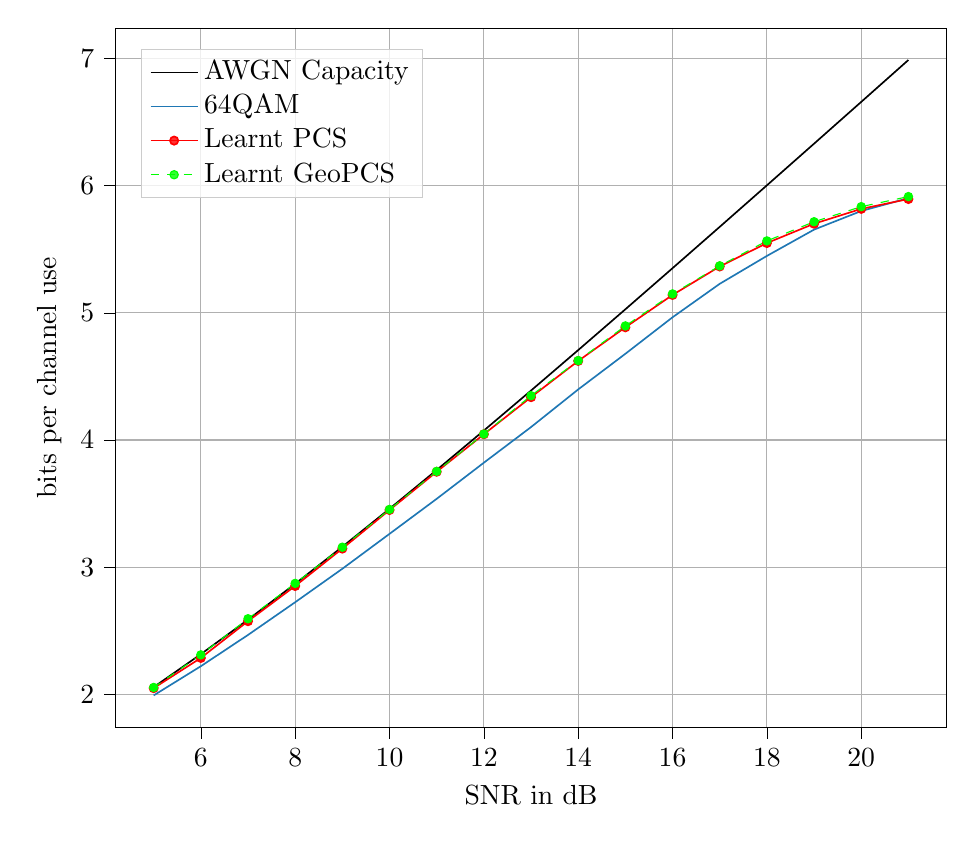
\begin{tikzpicture}

\definecolor{darkgray176}{RGB}{176,176,176}
\definecolor{lightgray204}{RGB}{204,204,204}
\definecolor{steelblue31119180}{RGB}{31,119,180}

\begin{axis}[
width=\textwidth,
legend cell align={left},
legend style={
  fill opacity=0.8,
  draw opacity=1,
  text opacity=1,
  at={(0.03,0.97)},
  anchor=north west,
  draw=lightgray204
},
tick align=outside,
tick pos=left,
x grid style={darkgray176},
xlabel={SNR in dB},
xmajorgrids,
xmin=4.2, xmax=21.8,
xtick style={color=black},
y grid style={darkgray176},
ylabel={bits per channel use},
ymajorgrids,
ymin=1.7427734204131, ymax=7.23721060364844,
ytick style={color=black}
]
\addplot [semithick, black]
table {%
5 2.0573732086068
6 2.31645617962626
7 2.58781437356203
8 2.86978721917029
9 3.16080442391302
10 3.4594316186373
11 3.76439436704286
12 4.07458523490543
13 4.38905896736305
14 4.70702026272884
15 5.02780767335052
16 5.3508761542486
17 5.67577990180488
18 6.00215644400198
19 6.32971245944191
20 6.65821148275179
21 6.98746345895592
};
\addlegendentry{AWGN Capacity}
\addplot [semithick, steelblue31119180]
table {%
5 1.99252056510562
6 2.22188472335438
7 2.46783010150158
8 2.72497762849336
9 2.98797481594902
10 3.26241611912443
11 3.53780680098415
12 3.82177960231084
13 4.10180988838577
14 4.3977281031029
15 4.67794065159212
16 4.96490024705524
17 5.22792292071708
18 5.44727967105006
19 5.65395561651234
20 5.80023460021518
21 5.90134552221041
};
\addlegendentry{64QAM}
\addplot [semithick, red, mark=*, mark size=1.5, mark options={solid}]
table {%
5 2.04953616842369
6 2.28690524728333
7 2.57595580065785
8 2.8524662390447
9 3.14655158452323
10 3.44979861779587
11 3.7504920526685
12 4.04539311186007
13 4.33694188522102
14 4.62174584298044
15 4.8859686369111
16 5.14053322913461
17 5.36437105698967
18 5.54836875980705
19 5.70036840250081
20 5.81702285871985
21 5.89450310672535
};
\addlegendentry{Learnt PCS}
\addplot [dashed, green, mark=*, mark size=1.5, mark options={solid}]
table {%
5 2.054870726288148
6 2.3113123371631734
7 2.5950424352506007
8 2.872956939999102
9 3.157409537202804
10 3.4543671649333914
11 3.7535450886866175
12 4.0472924882562
13 4.348614691700384
14 4.624498253324846
15 4.896956264509424
16 5.148696901605764
17 5.369250548759946
18 5.565256424225875
19 5.715805221276954
20 5.8343876030121615
21 5.913611755097416
};
\addlegendentry{Learnt GeoPCS}
\end{axis}

\end{tikzpicture}
\caption{Mutual information learned by the probabilistic constellation shpaing on the AWGN channel.}
\label{fig:arefPerf}
\end{figure}

